\newcommand{\aanleiding}{}

{\par \bigskip \par \color{red} TODO: Meer uitleg over begrippen \par \bigskip \par }

\begin{wrapfigure}{r}{4cm}
  \begin{center}
    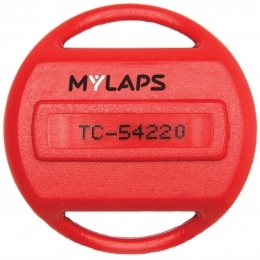
\includegraphics[width=4cm]{style/images/transponder}
  \end{center}
  \caption{MyLaps ProFlex transponder, op schaal} 
\end{wrapfigure}

In baansporten is de laatste jaren een ontwikkeling gaande om tijdregistratie te digitaliseren door het gebruik van transponders en detectie-lussen in de baan. Door deze ontwikkeling zijn nieuwe mogelijkheden ontstaan om ook naast het wedstrijdmoment de sportprestaties in te zien. Het constateren van de hierna genoemde nieuwe mogelijkheden was de aanleiding van dit project.

Een grote speler op de tijdregistratie-markt is MyLaps\footnote{\url{http://www.mylaps.com}}. Dit bedrijf installeert en beheert detectie-lussen en is actief bij diverse sporten zoals schaatsen, wielrennen, zwemmen, atletiek en diverse motorsporten. Bij sporten met permanente banen liggen de detectie-lussen het gehele jaar in de baan. Er bestaat de mogelijkheid om op de website van MyLaps doorkomst-tijden in te zien. De informatie die uit deze tijden is af te leiden, wordt door sporters als erg waardevol gezien om zich willen blijven verbeteren, waardoor er steeds meer getraind wordt met deze transponders.

\begin{figure}
  \label{fig:track-transponders}
  \begin{center}
    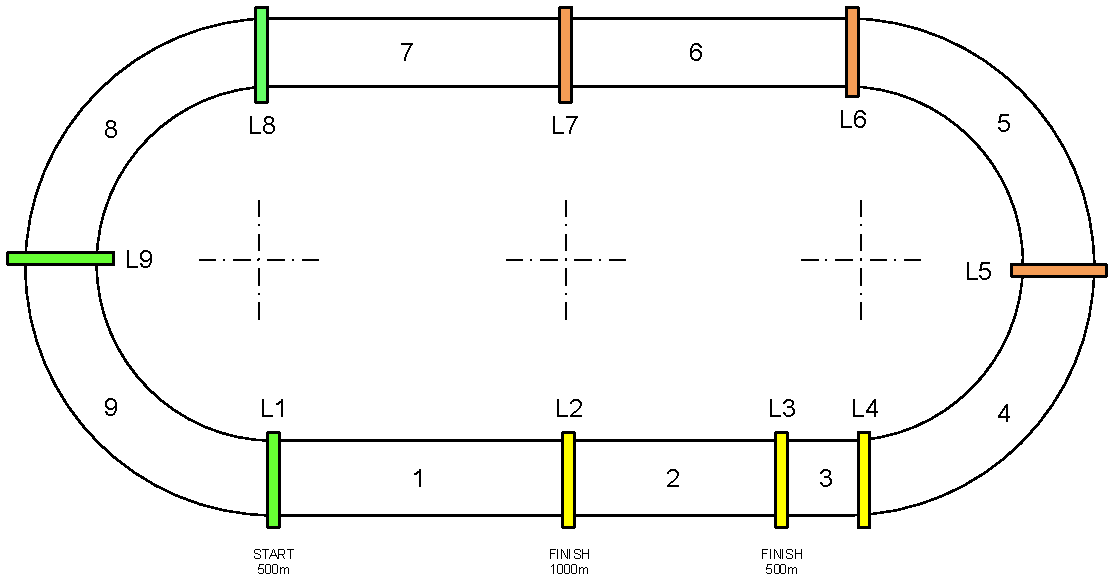
\includegraphics[width=\textwidth]{style/images/BaanoverzichtHaarlem}
  \end{center}
  \caption{L1 tot en met L9 zijn de negen MyLaps transponderlussen in Haarlem}
\end{figure}

Voor aanvang van het seizoen worden door MyLaps detectielussen geïnstalleerd. De lussen bevinden zich in het ijs of onder het houten oppervlak van een baanwielrenbaan. Elke lus heeft een elektromagnetisch veld. Wanneer een sporter met transponder over dat veld heen rijdt wordt de transponder geactiveerd en stuurt deze een unieke puls, die de lus opvangt. De MyLaps X2 server die aan de lussen zit aangesloten stuurt vervolgens het signaal door naar de MyLaps Cloud.

Het huidige gebruik van transponders - buiten wedstrijden - is voornamelijk achteraf, terwijl juist tijdens de training zowel sporter als coach het meeste bezig zijn met de prestaties. Het is daarom wenselijk om de resultaten in real-time door te geven aan coaches en sporters zelf.

Op de banen zijn meerdere detectie-lussen geïnstalleerd, terwijl er op de website van MyLaps slechts 1 wordt ontsloten. In Thialf\footnote{Schaatsbaan in Heerenveen, Friesland; van alle Nederlandse banen wordt deze baan het meeste gebruikt voor professionele wedstrijden.} liggen bijvoorbeeld 12 detectie-lussen en op de andere schaatsbanen liggen er tenminste 2. Door de data van meerdere lussen te combineren is een betere indicatie te maken van de snelheid van sporters.

\begin{wrapfigure}{r}{0.4\textwidth}
 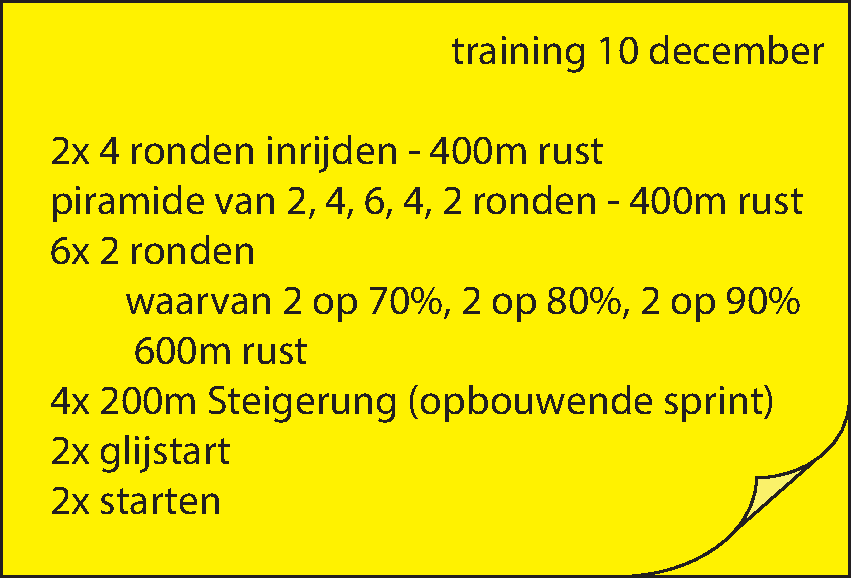
\includegraphics[width=0.4\textwidth]{style/images/training}
 \caption{Een typisch schaats-trainingsschema}
\end{wrapfigure}

Trainingen, bij bijvoorbeeld schaatsen, bestaan uit losse trainingsonderdelen. Allround schaatsers moeten bijvoorbeeld 4 ronden warmrijden, dan 6 keer 2 ronden sprinten, dan 4 keer een sprintje van 200 meter, 2 keer een glijstart en dan 2 keer een echte start bij de coach, vanuit de zijkant van de baan. Tussendoor is er rust, zo is het gebruikelijk om na een opdracht tenminste 400 meter uit te glijden. Het verschil tussen training en rust is af te leiden uit de verhouding tot de maximale snelheid.

Veel trainingselementen bestaan dus uit korte opdrachten, waar het juist om snelheid gaat. Een enkele lus is dan niet afdoende, omdat de rust voor of na de opdracht mee wordt gewogen. Sporters starten en stoppen namelijk niet precies boven de lus, maar starten vaak na de bocht en stoppen afhankelijk van de afstand van de opdracht op een willekeurig punt. 

Andere trainingen van bijvoorbeeld lange afstands- of marathonschaatsers kunnen bestaan uit één element: de hele training lang schaatsen, zonder overeind te komen. Wanneer er op tactische punten detectie-lussen geïnstalleerd zijn, is er bijvoorbeeld ook onderscheid te maken tussen bochten en de rechte stukken. Bij sporten met een ronde baan verschilt de snelheid in de bocht namelijk erg met die op het rechte eind. Deze vergelijking gebeurt nu al in Thialf, in het professionele circuit tijdens wedstrijden op televisie.

Topsporters zijn enorm prestatiegericht en als je al aan de top zit, dan kunnen kleine aanpassingen aan je techniek, ademhaling et cetera, grote verschillen maken. Coaches van professionele teams houden zich daarom bezig met allerhande analyses. Naast ademanalyse en hartslag monitoring, is het in Thialf bijvoorbeeld ook mogelijk om (van maximaal 20 schaatsers) continu de positie te bepalen met een in-door positioning system (IPS) ontwikkeld door InnoSportLab\footnote{\url{http://www.innosportlabthialf.nl}}.

Al deze geavanceerde analyses zijn echter te duur en kosten te veel tijd voor recreatieve sporters. MyLaps X2 biedt in combinatie met ons eindproduct recreatieve sporters toch een manier om analyses uit te voeren en zich naar een hoger niveau te tillen.